% modified from https://github.com/svmiller/svm-r-markdown-templates
\documentclass[]{article}
\usepackage[top=0.85in,right=2in]{geometry}
\newcommand*{\authorfont}{\fontfamily{phv}\selectfont}
\usepackage[]{mathpazo}


  \usepackage[T1]{fontenc}
  \usepackage[utf8]{inputenc}

\setlength{\parindent}{0pt}
\setlength{\parskip}{1em}

\renewcommand*{\thefootnote}{\fnsymbol{footnote}}

\usepackage{abstract}
\renewcommand{\abstractname}{}    % clear the title
\renewcommand{\absnamepos}{empty} % originally center

\renewenvironment{abstract}
 {{%
    \setlength{\leftmargin}{0mm}
    \setlength{\rightmargin}{\leftmargin}%
  }%
  \relax}
 {\endlist}

\makeatletter
\def\@maketitle{%
  \newpage
%  \null
%  \vskip 2em%
%  \begin{center}%
  \let \footnote \thanks
    {\fontsize{18}{20}\selectfont\raggedright  \setlength{\parindent}{0pt} \@title \par}%
}
%\fi
\makeatother




\setcounter{secnumdepth}{0}

\usepackage{color}
\usepackage{fancyvrb}
\newcommand{\VerbBar}{|}
\newcommand{\VERB}{\Verb[commandchars=\\\{\}]}
\DefineVerbatimEnvironment{Highlighting}{Verbatim}{commandchars=\\\{\}}
% Add ',fontsize=\small' for more characters per line
\usepackage{framed}
\definecolor{shadecolor}{RGB}{248,248,248}
\newenvironment{Shaded}{\begin{snugshade}}{\end{snugshade}}
\newcommand{\AlertTok}[1]{\textcolor[rgb]{0.94,0.16,0.16}{#1}}
\newcommand{\AnnotationTok}[1]{\textcolor[rgb]{0.56,0.35,0.01}{\textbf{\textit{#1}}}}
\newcommand{\AttributeTok}[1]{\textcolor[rgb]{0.77,0.63,0.00}{#1}}
\newcommand{\BaseNTok}[1]{\textcolor[rgb]{0.00,0.00,0.81}{#1}}
\newcommand{\BuiltInTok}[1]{#1}
\newcommand{\CharTok}[1]{\textcolor[rgb]{0.31,0.60,0.02}{#1}}
\newcommand{\CommentTok}[1]{\textcolor[rgb]{0.56,0.35,0.01}{\textit{#1}}}
\newcommand{\CommentVarTok}[1]{\textcolor[rgb]{0.56,0.35,0.01}{\textbf{\textit{#1}}}}
\newcommand{\ConstantTok}[1]{\textcolor[rgb]{0.00,0.00,0.00}{#1}}
\newcommand{\ControlFlowTok}[1]{\textcolor[rgb]{0.13,0.29,0.53}{\textbf{#1}}}
\newcommand{\DataTypeTok}[1]{\textcolor[rgb]{0.13,0.29,0.53}{#1}}
\newcommand{\DecValTok}[1]{\textcolor[rgb]{0.00,0.00,0.81}{#1}}
\newcommand{\DocumentationTok}[1]{\textcolor[rgb]{0.56,0.35,0.01}{\textbf{\textit{#1}}}}
\newcommand{\ErrorTok}[1]{\textcolor[rgb]{0.64,0.00,0.00}{\textbf{#1}}}
\newcommand{\ExtensionTok}[1]{#1}
\newcommand{\FloatTok}[1]{\textcolor[rgb]{0.00,0.00,0.81}{#1}}
\newcommand{\FunctionTok}[1]{\textcolor[rgb]{0.00,0.00,0.00}{#1}}
\newcommand{\ImportTok}[1]{#1}
\newcommand{\InformationTok}[1]{\textcolor[rgb]{0.56,0.35,0.01}{\textbf{\textit{#1}}}}
\newcommand{\KeywordTok}[1]{\textcolor[rgb]{0.13,0.29,0.53}{\textbf{#1}}}
\newcommand{\NormalTok}[1]{#1}
\newcommand{\OperatorTok}[1]{\textcolor[rgb]{0.81,0.36,0.00}{\textbf{#1}}}
\newcommand{\OtherTok}[1]{\textcolor[rgb]{0.56,0.35,0.01}{#1}}
\newcommand{\PreprocessorTok}[1]{\textcolor[rgb]{0.56,0.35,0.01}{\textit{#1}}}
\newcommand{\RegionMarkerTok}[1]{#1}
\newcommand{\SpecialCharTok}[1]{\textcolor[rgb]{0.00,0.00,0.00}{#1}}
\newcommand{\SpecialStringTok}[1]{\textcolor[rgb]{0.31,0.60,0.02}{#1}}
\newcommand{\StringTok}[1]{\textcolor[rgb]{0.31,0.60,0.02}{#1}}
\newcommand{\VariableTok}[1]{\textcolor[rgb]{0.00,0.00,0.00}{#1}}
\newcommand{\VerbatimStringTok}[1]{\textcolor[rgb]{0.31,0.60,0.02}{#1}}
\newcommand{\WarningTok}[1]{\textcolor[rgb]{0.56,0.35,0.01}{\textbf{\textit{#1}}}}

\usepackage{graphicx,grffile}
\usepackage[labelfont=bf]{caption}
\makeatletter
\def\maxwidth{\ifdim\Gin@nat@width>\linewidth\linewidth\else\Gin@nat@width\fi}
\def\maxheight{\ifdim\Gin@nat@height>\textheight\textheight\else\Gin@nat@height\fi}
\makeatother
% Scale images if necessary, so that they will not overflow the page
% margins by default, and it is still possible to overwrite the defaults
% using explicit options in \includegraphics[width, height, ...]{}
\setkeys{Gin}{width=\maxwidth,height=\maxheight,keepaspectratio}

\title{plyranges: A grammar of genomic data transformation  }



\author{\Large Stuart Lee
\footnote{\label{monash}Department of Econometrics and Business Statistics, Monash University, Clayton, Australia}\footnote{Molecular Medicine Division, Walter and Eliza Hall Institute, Parkville, Australia}\vspace{0.05in} \newline\normalsize\emph{}   \and \Large Dianne Cook \(^{\ref{monash}}\)\vspace{0.05in} \newline\normalsize\emph{}   \and \Large Michael Lawrence
\footnote{Bioinformatics and Computational Biology, Genentech Research and Early Development, South San Francisco, United States of America}\footnote{corresponding author}\vspace{0.05in} \newline\normalsize\emph{}  }


\date{}

\usepackage{titlesec}

\titleformat*{\section}{\normalsize\bfseries}
\titleformat*{\subsection}{\normalsize\itshape}
\titleformat*{\subsubsection}{\normalsize\itshape}
\titleformat*{\paragraph}{\normalsize\itshape}
\titleformat*{\subparagraph}{\normalsize\itshape}



% % 
% % \usepackage{biblatex}
% 
\usepackage[backend=biber, style=numeric-comp, url=false, sorting=none]{biblatex}
\addbibresource{references.bib}


\newtheorem{hypothesis}{Hypothesis}
\usepackage{setspace}

\makeatletter
\@ifpackageloaded{hyperref}{}{%
\ifxetex
  \PassOptionsToPackage{hyphens}{url}\usepackage[setpagesize=false, % page size defined by xetex
              unicode=false, % unicode breaks when used with xetex
              xetex]{hyperref}
\else
  \PassOptionsToPackage{hyphens}{url}\usepackage[unicode=true]{hyperref}
\fi
}

\@ifpackageloaded{color}{
    \PassOptionsToPackage{usenames,dvipsnames}{color}
}{%
    \usepackage[usenames,dvipsnames]{color}
}
\makeatother
\hypersetup{breaklinks=true,
            bookmarks=true,
            pdfauthor={Stuart Lee
\footnote{\label{monash}Department of Econometrics and Business Statistics, Monash University, Clayton, Australia}\footnote{Molecular Medicine Division, Walter and Eliza Hall Institute, Parkville, Australia} () and Dianne Cook \(^{\ref{monash}}\) () and Michael Lawrence
\footnote{Bioinformatics and Computational Biology, Genentech Research and Early Development, South San Francisco, United States of America}\footnote{corresponding author} ()},
             pdfkeywords = {Bioconductor, Grammar, Genomes, Data Analysis},  
            pdftitle={plyranges: A grammar of genomic data transformation},
            colorlinks=true,
            citecolor=blue,
            urlcolor=blue,
            linkcolor=magenta,
            pdfborder={0 0 0}}
\urlstyle{same}  % don't use monospace font for urls

% set default figure placement to htbp
\makeatletter
\def\fps@figure{htbp}
\makeatother



% add tightlist ----------
\providecommand{\tightlist}{%
\setlength{\itemsep}{0pt}\setlength{\parskip}{0pt}}

\begin{document}
	
% \pagenumbering{arabic}% resets `page` counter to 1 
%
% \maketitle

{% \usefont{T1}{pnc}{m}{n}
\setlength{\parindent}{0pt}
\thispagestyle{plain}
{\fontsize{18}{20}\selectfont\raggedright 
\maketitle  % title \par  

}

{
   \vskip 13.5pt\relax \normalsize\fontsize{11}{12} 
\textbf{\authorfont Stuart Lee
\footnote{\label{monash}Department of Econometrics and Business Statistics, Monash University, Clayton, Australia}\footnote{Molecular Medicine Division, Walter and Eliza Hall Institute, Parkville, Australia}} \hskip 15pt \emph{\small }   \par \textbf{\authorfont Dianne Cook \(^{\ref{monash}}\)} \hskip 15pt \emph{\small }   \par \textbf{\authorfont Michael Lawrence
\footnote{Bioinformatics and Computational Biology, Genentech Research and Early Development, South San Francisco, United States of America}\footnote{corresponding author}} \hskip 15pt \emph{\small }   

}

}








\begin{abstract}

    \hbox{\vrule height .2pt width 39.14pc}

    \vskip 8.5pt % \small 

\noindent The Bioconductor project has created many useful data abstractions for
analysing high-throughput genomics experiments. However, there is a
cognitive load placed on a user in learning a data abstraction and
understanding its appropriate use. Throughout a standard workflow, a
user must navigate and know many of these abstractions to perform an
genomic analysis task, when a single data abstraction, a GRanges object
will suffice. The GRanges class naturally represent genomic intervals
and their associated measurements. By recognising that the GRanges class
follows `tidy' data principles we have created a grammar of genomic data
transformation. The grammar defines verbs for performing actions on and
between genomic interval data. It provides a principled way of
performing common genomic data analysis tasks through a coherent
interface to existing Bioconductor infrastructure, resulting in human
readable analysis workflows. We have implemented this grammar as a
Bioconductor/R package called \texttt{plyranges}.


\vskip 8.5pt \noindent \emph{Keywords}: Bioconductor, Grammar, Genomes, Data Analysis \par

    \hbox{\vrule height .2pt width 39.14pc}



\end{abstract}


\vskip 6.5pt


\noindent  \hypertarget{background}{%
\section{Background}\label{background}}

High-throughput genomics promises to unlock new disease therapies, and
strengthen our knowledge of basic biology. To deliver on those promises,
scientists must derive a stream of knowledge from a deluge of data.
Genomic data is challenging in both scale and complexity. Innovations in
sequencing technology often outstrip our capacity to process the output.
Beyond their common association with genomic coordinates, genomic data
are heterogeneous, consisting of raw sequence read alignments, genomic
feature annotations like genes and exons, and summaries like coverage
vectors, ChIP-seq peak calls, variant calls, and per-feature read
counts. Genomic scientists need software tools to wrangle the different
types of data, process the data at scale, test hypotheses, and generate
new ones, all while focusing on the biology, not the computation. For
the tool developer, the challenge is to define ways to model and operate
on the data that align with the mental model of scientists, and to
provide an implementation that scales with their ambition.

Several domain specific languages (DSLs) enable scientists to process
and reason about heterogeneous genomics data by expressing common
operations, such as range manipulation and overlap-based joins, using
the vocabulary of genomics. Their implementations either delegate
computations to a database, or operate over collections of files in
standard formats like BED. An example of the former is the Genome Query
Language (GQL) and its distributed implementation GenAp which use an
SQL-like syntax for fast retrieval of information of unprocessed
sequencing data \autocites{Kozanitis2014-va}{Kozanitis2016-bm}.
Similarly, the Genometric Query Language (GMQL) implements a relational
algebra for combining genomic datasets \cite{Kaitoua2017-pw}. The
command line application BEDtools develops an extensive algebra for
performing arithmetic between two or more sets of genomic regions
\cite{Quinlan2010-gc}. All of the aforementioned DSLs are designed to be
evaluated either at the command line or embedded in scripts for batch
processing. They exist in a sparse ecosystem, mostly consisting of UNIX
and database tools that lack biological semantics and operate at the
level of files and database tables.

The Bioconductor/R packages \texttt{IRanges} and \texttt{GenomicRanges}
\autocites{r-core}{Lawrence2013-wg}{Huber2015-ei} define a DSL for
analysing genomics data with R, an interactive data analysis environment
that encourages reproducibility and provides high-level abstractions for
manipulating, modelling and plotting data, through state of the art
methods in statistical computing. The packages define object-oriented
(OO) abstractions for representing genomic data and enable
interoperability by allowing users and developers to use these
abstractions in their own code and packages. Other genomic DSLs that are
embedded in programming languages include pybedtools and valr
\autocites{Dale2011-js}{Kent2017}, however these packages lack the
interoperability provided by the aforementioned Bioconductor packages
and are not easily extended.

The Bioconductor infrastructure models the genomic data and operations
from the perspective of the power user, one who understands and wants to
take advantage of the subtle differences in data types. This design has
enabled the development of sophisticated tools, as evidenced by the
hundreds of packages depending on the framework. Unfortunately, the
myriad of data structures have overlapping purposes and important but
obscure differences in behavior that often confuse the typical end user.

Recently, there has been a concerted, community effort to standardize R
data structures and workflows around the notion of tidy data
\cite{Wickham2014-jc}. A tidy dataset is defined as a tabular data
structure that has observations as rows and columns as variables, and
all measurements pertain to a single observational unit. The tidy data
pattern is useful because it allows us to see how the data relate to the
design of an experiment and the variables measured. The \texttt{dplyr}
package \cite{Wickham2017-dplyr} defines an API that maps notions from
the general relational algebra to operations on tidy data. It expresses
each operation as a cohesive, endomorphic verb. Taken together these
features enable a user to write human readable analysis workflows.

We have created a genomic DSL called \texttt{plyranges} that
reformulates notions from existing genomic algebras and embeds them in R
as a genomic extension of \texttt{dplyr}. By analogy, \texttt{plyranges}
is to the genomic algebra, as \texttt{dplyr} is to the relational
algebra. The \texttt{plyranges} Bioconductor package implements the
language on top of a key subset of Bioconductor data structures and thus
fully integrates with the Bioconductor framework, gaining access to its
scalable data representations and sophisticated statistical methods.

\hypertarget{results}{%
\section{Results}\label{results}}

\hypertarget{genomic-relation-algebra}{%
\subsection{Genomic Relation Algebra}\label{genomic-relation-algebra}}

\hypertarget{data-model}{%
\subsubsection{Data Model}\label{data-model}}

\begin{figure}
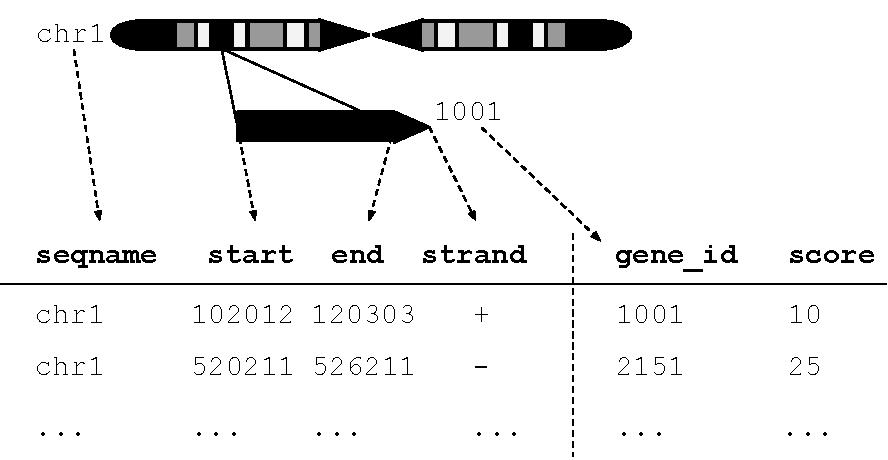
\includegraphics[width=\textwidth]{diagrams/GRanges}
\caption{An illustration of the GRanges data model for a
sample from an RNA-seq experiment. The core components of the data model
include a seqname column (representing the chromosome), a ranges column
which consists of start and end coordinates for a genomic region, and a
strand identifier (either positive, negative, or unstranded). Metadata
are included as columns to the right of the dotted line as annotations
(gene\_id) or range level covariates (score).}
\label{fig:GRanges} 
\end{figure}

The \texttt{plyranges} DSL is built on the core Bioconductor data
structure GRanges, which is essentially a constrained table, with fixed
columns for the chromosome, start and end coordinates, and the strand,
along with an arbitrary set of additional columns, consisting of
measurements or metadata specific to the data type or experiment (figure
\ref{fig:GRanges}). GRanges balances flexibility with formal
constraints, so that it is applicable to virtually any genomic workflow,
while also being semantically rich enough to support high-level
operations on genomic ranges. As a core data structure, GRanges enables
interoperability between \texttt{plyranges} and the rest of
Bioconductor. Adhering to a single data structure simplifies the API and
makes it easier to learn and understand, in part because operations
become endomorphic, i.e., they return the same type as their input.

GRanges follows the intuitive tidy data pattern: it is a rectangular
table corresponding to a single biological context. Each row contains a
single observation and each column is a variable describing the
observations. GRanges specializes the tidy pattern in that the
observations always pertain to some genomic feature, but it largely
remains compatible with the general relational operations defined by
dplyr. Thus, we define our algebra as an extension of the \texttt{dplyr}
algebra, and borrow its syntax conventions and design principles.

\begin{table}[!htbp]
\centering
\begin{tabular}{|l|l|p{6cm}|}
  \hline
  & Verb &  Description \\ 
  \hline
   & \textbf{\emph{summarise()}} & aggregate over column(s) \\ 
   Aggregation & \emph{disjoin\_ranges()} & aggregate column(s) over the union of end coordinates \\
   &  \emph{reduce\_ranges()} & aggregate column(s) by merging overlapping and neighbouring ranges \\
   \hline
   &  \textbf{\emph{mutate()}} & modifies any column \\
   & \textbf{\emph{select()}} & select columns \\
  Arithmetic (Unary) & \textbf{\emph{arrange()}} & sort by columns \\
   & \emph{stretch()} & extend range by fixed amount \\
   &  \emph{shift\_(direction)} & shift coordinates \\
   & \emph{flank\_(direction)} & generate flanking regions \\
   & \emph{\%intersection\% } & row-wise intersection \\
   & \emph{\%union\%} & row-wise union \\
   & \emph{compute\_coverage} & coverage over all ranges \\
  Arithmetic (Binary) &  \emph{\%setdiff\%} & row-wise set difference \\
   & \emph{between()} & row-wise gap range \\
   & \emph{span()} & row-wise spanning range \\
   \hline
    & \emph{join\_overlap\_*()} & merge by overlapping ranges \\
    & \emph{join\_nearest} & merge by nearest neighbour ranges \\
    & \emph{join\_follow} & merge by following ranges \\
    Merging & \emph{join\_precedes} & merge by preceding ranges \\
    & \emph{union\_ranges} & range-wise union \\
    & \emph{intersect\_ranges} & range-wise intersect \\
    & \emph{setdiff\_ranges} & range-wise set difference \\
    & \emph{complement\_ranges} & range-wise union \\
  \hline
   & \emph{anchor\_direction()} & fix coordinates at direction \\
  Modifier & \textbf{\emph{group\_by()}} & partition by column(s)  \\ 
   & \emph{group\_by\_overlaps()} & partition by overlaps \\
   \hline
   & \textbf{\emph{filter()}} & subset rows \\
  Restriction & \emph{filter\_by\_overlaps()} & subset by overlap \\
    & \emph{filter\_by\_non\_overlaps()} & subset by no overlap \\
   \hline
\end{tabular}
\caption{Overview of the \texttt{plyranges} grammar. The core verbs are
briefly described and categorised into one of: aggregation, unary or binary
arithmetic, merging, modifier, or restriction. A verb is given bold text if
its origin is from the \texttt{dplyr} grammar.}\label{tab:grammar}
\end{table}

\hypertarget{algebraic-operations}{%
\subsubsection{Algebraic operations}\label{algebraic-operations}}

The \texttt{plyranges} DSL defines an expressive algebra for performing
genomic operations with and between GRanges objects (see table
\ref{tab:grammar}). The grammar includes several classes of operation
that cover most use cases in genomics data analysis. There are range
arithmetic operators, such as for resizing ranges or finding their
intersection, and operators for merging, filtering and aggregating by
range-specific notions like overlap and proximity.

Arithmetic operations transform range coordinates, as defined by their
\emph{start}, \emph{end} and \emph{width}. The three dimensions are
mutually dependent and partially redundant, so direct manipulation of
them is problematic. For example, changing the \emph{width} column needs
to change either the \emph{start}, \emph{end} or both to preserve
integrity of the object. We introduce the \emph{anchor} modifier to
disambiguate these adjustments. Supported anchor points include the
start, end and midpoint, as well as the 3' and 5' ends for
strand-directed ranges. For example, if we anchor the start, then
setting the width will adjust the end while leaving the start
stationary.

The algebra also defines conveniences for relative coordinate
adjustments: \emph{shift} (unanchored adjustment to both start and end)
and \emph{stretch} (anchored adjustment of width). We can perform any
relative adjustment by some combination of those two operations. The
\emph{stretch} operation requires an anchor and assumes the midpoint by
default. Since \emph{shift} is unanchored, the user specifies a suffix
for indicating the direction: left/right or, for stranded features,
upstream/downstream. For example, \emph{shift\_right} shifts a range to
the right.

The \emph{flank} operation generates new ranges that are adjacent to
existing ones. This is useful, for example, when generating upstream
promoter regions for genes. Analogous to \emph{shift}, a suffix
indicates the side of the input range to flank.

As with other genomic grammars, we define set operations that treat
ranges as sets of integers, including \emph{intersect}, \emph{union},
\emph{difference}, and \emph{complement}. There are two sets of these:
parallel and merging. For example, the parallel intersection (\emph{x
\%intersect\% y}) finds the intersecting range between \emph{xi} and
\emph{yi} for \emph{i} in \emph{1\ldots{}n}, where \emph{n} is the
length of both \emph{x} and \emph{y}. In contrast, the merging
intersection (\emph{intersect\_ranges(x, y)}) returns a new set of
disjoint ranges representing wherever there was overlap between a range
in \emph{x} and a range in \emph{y}. Finding the parallel union will
fail when two ranges have a gap, so we introduce a \emph{span} operator
that takes the union while filling any gap. The \emph{complement}
operation is unique in that it is unary. It finds the regions not
covered by any of the ranges in a single set. Closely related is the
\emph{between} parallel operation, which finds the gap separating
\emph{xi} and \emph{yi}. The binary operations are callable from within
arithmetic, restriction and aggregation expressions.

To support merging, our algebra recasts finding overlaps or nearest
neighbours between two genomic regions as variants of the relational
join operator. A join acts on two GRanges objects, a query and a
subject. The join operator is relational in the sense that metadata from
the query and subject ranges is retained in the joined range. All join
operators in the \texttt{plyranges} DSL generate a set of hits based on
overlap or proximity of ranges and use those hits to merge the two
datasets in different ways. There are four supported matching
algorithms: \emph{overlap}, \emph{nearest}, \emph{precede}, and
\emph{follow} (figures \ref{fig:olaps-fig} and \ref{fig:nn-fig}). We can
further restrict the matching by whether the query is completely
\emph{within} the subject, and adding the \emph{directed} suffix ensures
that matching ranges have the same direction (strand).

\begin{figure}

{\centering 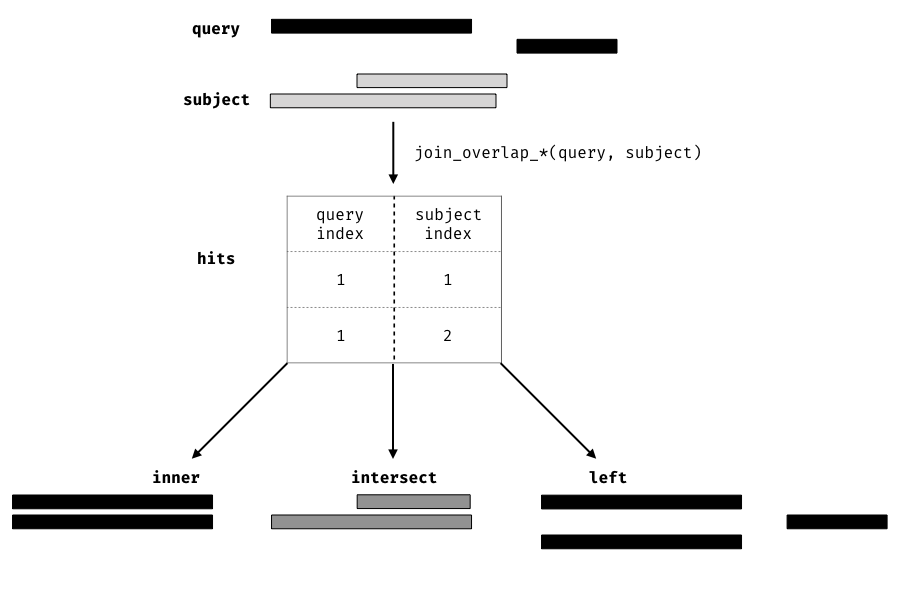
\includegraphics[width=\textwidth]{diagrams/diagrams-002} 

}

\caption{Illustration of the three overlap join operators. Each join takes query and subject range as input (black and light gray rectangles, respectively). An index for the join is computed, returning a Hits object, which contains the indices of where the subject overlaps the query range. This index is used to expand the query ranges by where it was 'hit' by the subject ranges. The join semantics alter what is returned: for an \textbf{inner} join the query range is returned for each match, for an \textbf{intersect} the intersection is taken between overlapping ranges, and for a \textbf{left} join all query ranges are returned even if the subject range does not overlap them. This principle is gnerally applied through the `plyranges` DSL for both overlaps and nearest neighbour operations.}\label{fig:olaps-fig}
\end{figure}

For merging based on the hits, we have three modes: \emph{inner},
\emph{intersect} and \emph{left}. The \emph{inner} overlap join is
similar to the conventional inner join in that there is a row in the
result for every match. A major difference is that the matching is not
by identity, so we have to choose one of the ranges from each pair. We
always choose the left range. The \emph{intersect} join uses the
intersection instead of the left range. Finally, the overlap \emph{left}
join is akin to left outer join in Cobb's relational algebra: it
performs an overlap inner join but also returns all query ranges that
are not hit by the subject.

\begin{figure}

{\centering 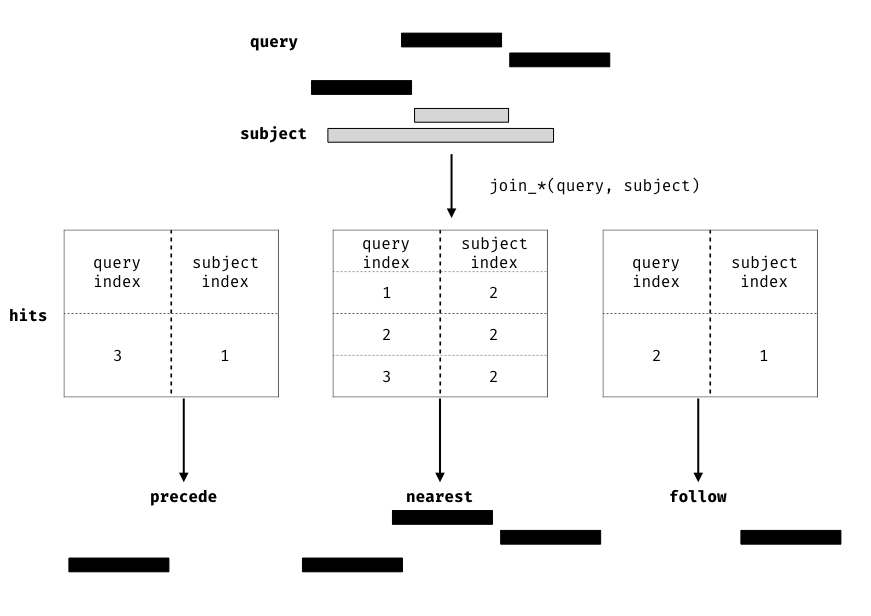
\includegraphics[width=\textwidth]{diagrams/diagrams-003} 

}

\caption{Illustration of neighbour finding joins. Each join takes a query and subject range and computes a 'Hits' object. For the \textbf{nearest} join all query ranges are returned as they are all nearest neighbours of the second subject range. For the \textbf{follow} join there is only one query range that follows any subject range. Likewise for the \textbf{precede} join, there is only one query range that precedes a subject range.}\label{fig:nn-fig}
\end{figure}

Since the GRanges object is a tabular data structure, our grammar
includes operators to filter, sort and aggregate by columns in a
GRanges. These operations can be performed over partitions formed using
the \emph{group\_by} modifier. Together with our algebra for arithmetic
and merging, these operations conform to the semantics and syntax of the
\texttt{dplyr} grammar.

\hypertarget{developing-workflows-with-plyranges}{%
\subsection{\texorpdfstring{Developing workflows with
\texttt{plyranges}}{Developing workflows with plyranges}}\label{developing-workflows-with-plyranges}}

Here we provide illustrative examples of using the \texttt{plyranges}
DSL to show how our grammar could be integrated into genomic data
workflows. We also highlight how interoperability with existing
Bioconductor infrastructure, enables easy access to public datasets and
methods for analysis and visualisation.

\hypertarget{peak-finding}{%
\subsubsection{Peak Finding}\label{peak-finding}}

In the workflow of ChIP-seq data analysis, we are interested in finding
peaks from islands of coverage over chromosome. Here we will use
\texttt{plyranges} to call peaks from islands of coverage above 8 then
plot the region surrounding the tallest peak.

Using \texttt{plyranges} and the the Bioconductor package
\texttt{AnnotationHub} \cite{R-ahub} we can download and read BigWig
files from ChIP-Seq experiments from the Human Epigenome Roadmap project
\cite{Roadmap-Epigenomics-Consortium2015-pr}. Here we analyse a BigWig
file corresponding to H3 lysine 27 trimethylation (H3K27Me3) of primary
T CD8+ memory cells from peripheral blood, focussing on coverage islands
over chromosome 10.

First, we extract the genome information from the BigWig file and filter
to get the range for chromosome 10. This range will be used as a filter
when reading the file.

\begin{Shaded}
\begin{Highlighting}[]
\KeywordTok{library}\NormalTok{(plyranges)}
\NormalTok{chr10_ranges <-}\StringTok{ }\NormalTok{bw_file }\OperatorTok\StringTok{ }
\StringTok{  }\KeywordTok{get_genome_info}\NormalTok{() }\OperatorTok
\StringTok{  }\KeywordTok{filter}\NormalTok{(seqnames }\OperatorTok{==}\StringTok{ "chr10"}\NormalTok{)}
\end{Highlighting}
\end{Shaded}

Then we read the BigWig file only extracting scores if they overlap
chromosome 10. We also add the genome build information to the resulting
ranges. This book-keeping is good practice as it ensures the integrity
of any downstream operations such as finding overlaps.

\begin{Shaded}
\begin{Highlighting}[]
\NormalTok{chr10_scores <-}\StringTok{ }\NormalTok{bw_file }\OperatorTok
\StringTok{  }\KeywordTok{read_bigwig}\NormalTok{(}\DataTypeTok{overlap_ranges =}\NormalTok{ chr10_ranges) }\OperatorTok
\StringTok{  }\KeywordTok{set_genome_info}\NormalTok{(}\DataTypeTok{genome =} \StringTok{"hg19"}\NormalTok{)}
\end{Highlighting}
\end{Shaded}

After filtering for regions with a coverage score greater than 8, we can
reduce individual runs to ranges representing the islands of coverage by
using the \texttt{reduce\_ranges()} function. This function allows a
summary to be computer over each island: in this case we take the
maximum of the scores to find the coverage peaks over chromosome 10.

\begin{Shaded}
\begin{Highlighting}[]
\NormalTok{all_peaks <-}\StringTok{ }\NormalTok{chr10_scores }\OperatorTok\StringTok{ }
\StringTok{  }\KeywordTok{filter}\NormalTok{(score }\OperatorTok{>}\StringTok{ }\DecValTok{8}\NormalTok{) }\OperatorTok\StringTok{ }
\StringTok{  }\KeywordTok{reduce_ranges}\NormalTok{(}\DataTypeTok{score =} \KeywordTok{max}\NormalTok{(score))}
\end{Highlighting}
\end{Shaded}

Returning to the GRanges object containing normalised coverage scores,
we filter to find the coordinates of the peak containing the maximum
coverage score. We can then find a 5000 nt region centered around the
maximum position by anchoring and modifying the width.

\begin{Shaded}
\begin{Highlighting}[]
\NormalTok{chr10_max_score_region <-}\StringTok{ }\NormalTok{chr10_scores }\OperatorTok
\StringTok{  }\KeywordTok{filter}\NormalTok{(score }\OperatorTok{==}\StringTok{ }\KeywordTok{max}\NormalTok{(score)) }\OperatorTok\StringTok{ }
\StringTok{  }\KeywordTok{anchor_center}\NormalTok{() }\OperatorTok
\StringTok{  }\KeywordTok{mutate}\NormalTok{(}\DataTypeTok{width =} \DecValTok{5000}\NormalTok{)}
\end{Highlighting}
\end{Shaded}

Finally, the overlap inner join is used to restrict the chromosome 10
coverage islands, to the islands that are contained in the 5000nt region
that surrounds the max peak (figure \ref{fig:peak-viz}).

\begin{Shaded}
\begin{Highlighting}[]
\NormalTok{peak_region <-}\StringTok{ }\NormalTok{chr10_scores }\OperatorTok
\StringTok{  }\KeywordTok{join_overlap_inner}\NormalTok{(chr10_max_score_region)}
\end{Highlighting}
\end{Shaded}

\begin{figure}

{\centering 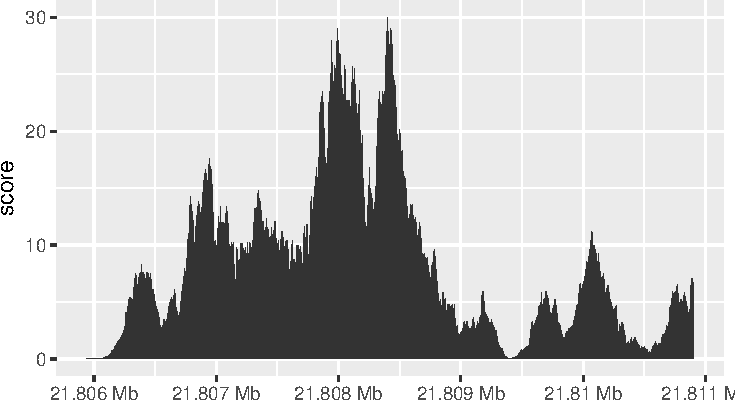
\includegraphics{paper_files/figure-latex/peak-viz-1} 

}

\caption{The final result of the \texttt{plyranges} operations to find a 5000nt region surrounding the peak of normalised coverage scores over chromosome 10, displayed as a density plot.}\label{fig:peak-viz}
\end{figure}

\hypertarget{computing-windowed-statistics}{%
\subsubsection{Computing Windowed
Statistics}\label{computing-windowed-statistics}}

Another common operation in genomics data analysis is to compute data
summaries over genomic windows. In \texttt{plyranges} this can be
achieved via the \texttt{group\_by\_overlaps()} operator. We bin and
count and find the average GC content of reads from a H3K27Me3 ChIP-seq
experiment by the Human Epigenome Roadmap Consortium.

We can directly obtain the genome information from the header of the BAM
file: in this case the reads were aligned to the hg19 genome build and
there are no reads overlapping the mitochondrial genome. To generate
bins of fixed width 10000nt we apply the \texttt{tile\_ranges()}
function to the genomic coordinates in locations.

\begin{Shaded}
\begin{Highlighting}[]
\NormalTok{locations <-}\StringTok{ }\NormalTok{h1_bam_sorted }\OperatorTok
\StringTok{  }\KeywordTok{read_bam}\NormalTok{() }\OperatorTok\StringTok{ }
\StringTok{  }\KeywordTok{get_genome_info}\NormalTok{() }

\NormalTok{bins <-}\StringTok{ }\NormalTok{locations }\OperatorTok\StringTok{ }
\StringTok{  }\KeywordTok{tile_ranges}\NormalTok{(}\DataTypeTok{width =}\NormalTok{ 10000L)}
\end{Highlighting}
\end{Shaded}

Next we only read in alignments that overlap the genomic locations we
are interested in and select the query sequence. Note that the reading
of the BAM file is deferred: only alignments that pass the filter are
loaded into memory. We can add another column representing the GC
proportion for each alignment using the \texttt{letterFrequency()}
function from the \texttt{Biostrings} package \cite{R-biostrings}.

\begin{Shaded}
\begin{Highlighting}[]
\NormalTok{alignments <-}\StringTok{ }\NormalTok{h1_bam_sorted }\OperatorTok\StringTok{ }
\StringTok{  }\KeywordTok{read_bam}\NormalTok{() }\OperatorTok
\StringTok{  }\KeywordTok{filter_by_overlaps}\NormalTok{(locations) }\OperatorTok
\StringTok{  }\KeywordTok{select}\NormalTok{(seq) }\OperatorTok
\StringTok{  }\KeywordTok{mutate}\NormalTok{(}\DataTypeTok{score =} \KeywordTok{as.numeric}\NormalTok{(}\KeywordTok{letterFrequency}\NormalTok{(seq, }\StringTok{"GC"}\NormalTok{, }\DataTypeTok{as.prob =} \OtherTok{TRUE}\NormalTok{)))}
\end{Highlighting}
\end{Shaded}

Finally, we use \texttt{group\_by\_overlaps()} to see where the
alignments overlap the genomic windows and then apply
\texttt{summarize()} to compute the total number of reads and average GC
content within each window.

\begin{Shaded}
\begin{Highlighting}[]
\NormalTok{alignments_summary <-}\StringTok{ }\NormalTok{bins }\OperatorTok
\StringTok{  }\KeywordTok{group_by_overlaps}\NormalTok{(alignments }\OperatorTok\StringTok{ }\KeywordTok{select}\NormalTok{(score)) }\OperatorTok\StringTok{ }
\StringTok{  }\KeywordTok{summarize}\NormalTok{(}\DataTypeTok{n_reads =} \KeywordTok{n}\NormalTok{(), }\DataTypeTok{avg_gc =} \KeywordTok{mean}\NormalTok{(score))}
\end{Highlighting}
\end{Shaded}

\hypertarget{quality-control-metrics}{%
\subsubsection{Quality Control Metrics}\label{quality-control-metrics}}

We have created a GRanges object from genotyping performed on the H1
cell line, consisting of approximately two million single nucleotide
polymorphisms (SNPs) and short insertion/deletions (indels). The GRanges
object consists of 7 columns, relating to the alleles of a SNP or indel,
the B-allele frequency, log relative intensity of the probes, GC content
score over a probe, and the name of the probe. We can use this
information to compute the transition-transversion ratio, a quality
control metric, within each chromosome in GRanges object.

First we filter out the indels and mitochondrial variants. Then we
create a logical vector corresponding to whether there is a transition
event.

\begin{Shaded}
\begin{Highlighting}[]
\NormalTok{h1_snp_array <-}\StringTok{ }\NormalTok{h1_snp_array }\OperatorTok
\StringTok{  }\KeywordTok{filter}\NormalTok{(}\OperatorTok{!}\NormalTok{(ref }\OperatorTok\StringTok{ }\KeywordTok{c}\NormalTok{(}\StringTok{"I"}\NormalTok{, }\StringTok{"D"}\NormalTok{)), seqnames }\OperatorTok{!=}\StringTok{ "M"}\NormalTok{) }\OperatorTok
\StringTok{  }\KeywordTok{mutate}\NormalTok{(}\DataTypeTok{transition =}\NormalTok{ (ref }\OperatorTok\StringTok{ }\KeywordTok{c}\NormalTok{(}\StringTok{"A"}\NormalTok{, }\StringTok{"G"}\NormalTok{) }\OperatorTok{&}\StringTok{ }\NormalTok{alt }\OperatorTok\StringTok{ }\KeywordTok{c}\NormalTok{(}\StringTok{"G"}\NormalTok{,}\StringTok{"A"}\NormalTok{))}\OperatorTok{|}
\StringTok{                      }\NormalTok{(ref }\OperatorTok\StringTok{ }\KeywordTok{c}\NormalTok{(}\StringTok{"C"}\NormalTok{,}\StringTok{"T"}\NormalTok{) }\OperatorTok{&}\StringTok{ }\NormalTok{alt }\OperatorTok\StringTok{ }\KeywordTok{c}\NormalTok{(}\StringTok{"T"}\NormalTok{, }\StringTok{"C"}\NormalTok{)))}
\end{Highlighting}
\end{Shaded}

We then compute the transition-transversion ratio over each chromosome
using \texttt{group\_by()} in combination with \texttt{summarize()}
(figure \ref{fig:titv-viz}).

\begin{Shaded}
\begin{Highlighting}[]
\NormalTok{ti_tv_results <-}\StringTok{ }\NormalTok{h1_snp_array }\OperatorTok\StringTok{ }
\StringTok{  }\KeywordTok{group_by}\NormalTok{(seqnames) }\OperatorTok
\StringTok{  }\KeywordTok{summarize}\NormalTok{(}\DataTypeTok{n_snps =} \KeywordTok{n}\NormalTok{(),}
            \DataTypeTok{ti_tv =} \KeywordTok{sum}\NormalTok{(transition) }\OperatorTok{/}\StringTok{ }\KeywordTok{sum}\NormalTok{(}\OperatorTok{!}\NormalTok{transition)) }
\end{Highlighting}
\end{Shaded}

\begin{figure}

{\centering 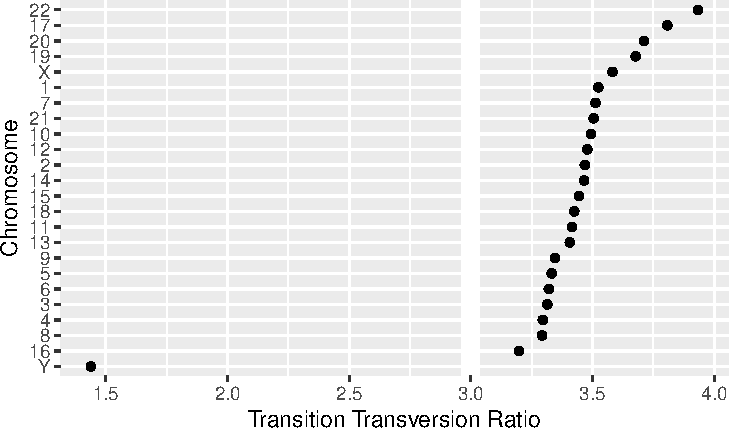
\includegraphics{paper_files/figure-latex/titv-viz-1} 

}

\caption{The final result of computing quality control metrics over the SNP array data with \texttt{plyranges}, displayed as a dot plot. Chromosomes are ordered by their estimated transition-transversion ratio. A white reference line is drawn at the expected ratio for a human exome.}\label{fig:titv-viz}
\end{figure}

\hypertarget{discussion}{%
\section{Discussion}\label{discussion}}

The design of \texttt{plyranges} adheres to well understood principles
of language and API design: cognitive consistency, cohesion,
expressiveness and endomorphism \cite{Green1996-qg}. To varying degrees,
these principles also underlie the design of \texttt{dplyr} and the
Bioconductor infrastructure.

We have aimed for \texttt{plyranges} to have a simple and direct mapping
to the user's cognitive model, i.e., how the user thinks about the data.
This requires careful selection of the level of abstraction so that the
user can express workflows in the language of genomics. This motivates
the adoption of the tidy GRanges object as our central data structure.
The basic data.frame and \texttt{dplyr} tibble lack any notion of
genomic ranges and so could not easily support our genomic grammar, with
its specific verbs for range-oriented data manipulation. Another example
of cognitive consistency is how \texttt{plyranges} is insensitive to
direction/strand by default when, e.g., detecting overlaps.
\texttt{GenomicRanges} has the opposite behavior. We believe that
defaulting to purely spatial overlap is most intuitive to most users.

Like \texttt{dplyr}, \texttt{plyranges} verbs are functional: they are
free of side effects and return their result. This enables chaining of
verbs through syntax like the forward pipe operator
(\texttt{\%\textgreater{}\%}, read as ``then'') of the \texttt{magrittr}
package \cite{R-magrittr}. This has syntax has a direct cognitive
mapping to natural language and the intuitive notion of pipelines. The
low-level object-oriented APIs of Bioconductor tend to manipulate data
via sub-replacement functions, like \texttt{start(gr)\ \textless{}-\ x}.
These ultimately produce the side effect of replacing a symbol mapping
in the current environment and thus are not amenable to so-called fluent
syntax.

A function is cohesive if it performs a singular task without producing
any side-effects. Singular tasks can always be broken down further at
lower levels of abstraction. For example, to resize a range, the user
needs to specify which position (start, end, midpoint) should be
invariant over the transformation. The \texttt{resize()} function from
the \texttt{GenomicRanges} package has a \texttt{fix} argument that sets
the anchor, so calling \texttt{resize()} coalesces anchoring and width
modification. The coupling at the function call level is justified since
the effect of setting the width depends on the anchor. However,
\texttt{plyranges} increases cohesion and decouples the anchoring into
its own function call.

Increasing cohesion simplifies the interface to each operation, makes
the meaning of arguments more intuitive, and relies on function names as
the primary means of expression, instead of a more complex mixture of
function and argument names. This results in the user being able to
conceptualize the \texttt{plyranges} DSL as a flat catalog of functions,
without having to descend further into documentation to understand a
function's arguments. A flat function catalog also enhances API
discoverability, particularly through auto-completion in IDEs. One
downside of pushing cohesion to this extreme is that function calls
become coupled, and care is necessary to treat them as a group when
modifying code.

Expressiveness relates to the information content in code: the
programmer should be able to clarify intent without unnecessary
verbosity. For example, our overlap-based join operations are more
concise than the multiple steps necessary to achieve the same effect in
the original \texttt{GenomicRanges} API. In other cases, the
\texttt{plyranges} API increases verbosity for the sake of clarity and
cohesion. Explicitly calling \emph{anchor()} can require more typing,
but the code is easier to comprehend. Another example is the set of
routines for importing genomic annotations, including
\emph{read\_gff()}, \emph{read\_bed()}, and \emph{read\_bam()}. Compared
to the generic \emph{import()} in \texttt{rtracklayer}, the explicit
format-based naming in \texttt{plyranges} clarifies intent and the type
of data being returned. Similarly, every \texttt{plyranges} function
that computes with strand information indicates its intentions by
including suffixes such as \emph{directed}, \emph{upstream} or
\emph{downstream} in its name, otherwise strand is ignored. The
\texttt{GenomicRanges} API does not make this distinction explicit in
its function naming, instead relying on a parameter that defaults to
strand sensitivity, an arguably unintuitive behavior.

A caveat to constructing a compatible interface with \texttt{dplyr} is
that \texttt{plyranges} makes extensive use of non-standard evaluation
in R via the \texttt{rlang} package \cite{R-rlang}. Simply, this means
that computations are evaluated in the context of the GRanges objects.
Both \texttt{dplyr} and \texttt{plyranges} are based on the
\texttt{rlang} language, because it allows for more expressive code that
is free of repeated references to the container. Implicitly referencing
the container is particularly convenient when programming interactively.
Consequently, when programming with \texttt{plyranges}, a user needs to
generally understand the \texttt{rlang} language and how to adapt their
code accordingly. Users familiar with the tidyverse should already have
such knowledge.

\hypertarget{conclusion}{%
\section{Conclusion}\label{conclusion}}

We have shown how to create expressive and reproducible genomic
workflows using the \texttt{plyranges} DSL. By realising that the
GRanges data model is tidy we have highlighted how to implement a
grammar for performing genomic arithmetic, aggregation, restriction and
merging. Our examples show that \texttt{plyranges} code is succinct,
human readable and can take advantage of the interoperability provided
by the Bioconductor ecosystem and the R language.

We aim to continue developing the \texttt{plyranges} package and to
extend it for use with more complex data structures, such as the
SummarizedExperiment class, the core Bioconductor data structure for
representing experimental results (e.g., counts) from multiple sample
experiments in conjunction with feature and sample metadata. The grammar
and design of the \texttt{plryanges} DSL are naturally extensible to
SummarizedExperiment.

As the \texttt{plyranges} interface encourages tidy data practices, it
integrates well with the grammar of graphics \cite{Wickham2016-gz}. To
achieve responsive performance, interactive graphics rely on lazy data
access and computing patterns, so the deferred mechanisms within
\texttt{plyranges} should help support interactive genomics
applications.

The \texttt{plyranges} package can be obtained via the Bioconductor
project website \url{https://bioconductor.org} or accessed via Github
\url{https://github.com/sa-lee/plyranges}.

\hypertarget{methods}{%
\section{Methods}\label{methods}}

\hypertarget{data-availability}{%
\subsection{Data Availability}\label{data-availability}}

The BigWig file for the H3K27Me3 primary T CD8+ memory cells from
peripheral blood ChIP-seq data was downloaded from the
\texttt{AnnotationHub} package (2.12.0) under accession AH33458. The BAM
file corresponding to the H1 cell line ChIP-seq data is available at GEO
under accession GSM433167. The SNP array data for the H1 cell line data
is available at GEO under accession GSM1463263.

\hypertarget{software-versions}{%
\subsection{Software Versions}\label{software-versions}}

To produce the workflows as described in results section we used R
version 3.5 with the development version of \texttt{plyranges} (1.1.4)
and the \texttt{BioStrings} package (2.48.0) installed.

All code required to reproduce this article is available at
\url{https://github.com/sa-lee/plyranges-paper}.

\hypertarget{acknowledgements}{%
\section{Acknowledgements}\label{acknowledgements}}

We would like to thank Dr Matthew Ritchie at the Walter and Eliza Hall
Institute and Dr Paul Harrison for their feedback on earlier drafts of
this work. We would also like to thank Lori Shepherd and Hèrve Pages for
the code review they performed. This article was written with
\texttt{knitr} \cite{R-knitr} and the figures were made with
\texttt{ggbio} \cite{R-ggbio}.




\newpage
\singlespacing 
\printbibliography[title=References]

\end{document}
